\documentclass[12pt]{article}
\usepackage{amsmath}
\usepackage{siunitx}
\usepackage{longtable}
\usepackage{tikz}

\begin{document}
	
	\title{Projectile Motion Problem}
	\author{}
	\date{}
	\maketitle
	
	\section*{Problem Statement}
\textit{	A ball is rolled off a desk that is 1.2 m tall, aiming to hit a target 3.5 m away from the base of the desk. The ball rolls horizontally off the edge.  
	What must the initial horizontal velocity of the ball (\(v_{ix}\)) be to hit the target?}
	
	\section*{Step 1: Diagram}
	
	\begin{center}
		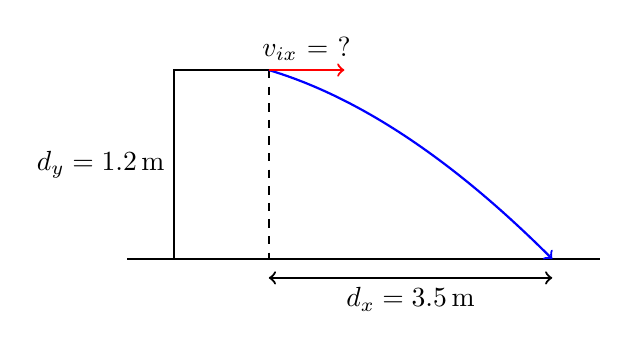
\begin{tikzpicture}[scale=1.2]
			% Draw the desk
			\draw[thick] (0,0) -- (0,2) -- (1,2);
			\draw[thick, dashed] (1,2) -- (1,0); % dashed line to the ground
			\node[anchor=east] at (0,1) {$d_y = 1.2\,\text{m}$}; % label for height
			
			% Draw the ground
			\draw[thick] (-0.5,0) -- (4.5,0);
			
			% Draw the projectile path
			\draw[thick, ->, color=blue] (1,2) .. controls (2,1.7) and (3,1) .. (4,0);
			
			% Draw the horizontal distance
			\draw[<->, thick] (1,-0.2) -- (4,-0.2);
			\node[anchor=north] at (2.5,-0.2) {$d_x = 3.5\,\text{m}$};
			
			% Initial velocity vector
			\draw[->, thick, color=red] (1,2) -- (1.8,2);
			\node[anchor=south] at (1.4,2) {$v_{ix}$ = ?};
			
			% Gravity arrow
		%	\draw[->, thick, color=green] (3,1) -- (3,0.2);
		%	\node[anchor=west] at (3,0.6) {$a_y = 9.81\,\text{m/s}^2$};
			
			% Label for ball
		%	\filldraw[blue] (1,2) circle (0.05) node[anchor=south west] {Ball};
		\end{tikzpicture}
	\end{center}
	
	\section*{Step 2: Understand the Variables and Known Values}
	
	\begin{longtable}{|c l | c l|}
		\hline
		\multicolumn{2}{|c|}{\textbf{Horizontal}} & \multicolumn{2}{|c|}{\textbf{Vertical}} \\
		\hline
		\(d_x = \) & \(\SI{3.5}{m}\) & \(d_y = \) & \(\SI{1.2}{m}\) \\
		\hline
		\(v_{ix} = \) & ? & \(v_{iy} = \) & \(\SI{0}{m/s}\) \\
		\hline
		\(v_{fx} = \) & ? & \(v_{fy} = \) & ? \\
		\hline
		\(a_x = \) & \(\SI{0}{m/s^2}\) & \(a_y = \) & \(\SI{9.81}{m/s^2}\) \\ 
		\hline
		\multicolumn{2}{|r|}{\(t =\)} & \multicolumn{2}{l|}{?}  \\
		\hline
	\end{longtable}
	
	\section*{Step 3: Use Vertical Motion to Find Time (\(t\))}
	
	The vertical motion equation is:
	\[
	d_y = v_{iy}t + \frac{1}{2}a_y t^2
	\]
	
	Substitute \(v_{iy} = 0\):
	\[
	d_y = \frac{1}{2}a_y t^2
	\]
	
	Rearrange to solve for \(t\):
	\[
	t = \sqrt{\frac{2d_y}{a_y}}
	\]
	
	Substitute \(d_y = 1.2 \, \text{m}\) and \(a_y = 9.81 \, \text{m/s}^2\):
	\[
	t = \sqrt{\frac{2(1.2)}{9.81}} = \sqrt{0.2445} \approx 0.494 \, \text{seconds}
	\]
	
	\section*{Step 4: Find Initial Horizontal Velocity}
	
	The horizontal motion equation is:
	\[
	d_x = v_{ix} t + \frac{1}{2}a_xt^2
	\]
	Since $a_x = \SI{0}{m/s^2}$ , the equation becomes:
	\[ d_x = v_{ix} t \]
	
	
	Rearrange to solve for \(v_{ix}\):
	\[
	v_{ix} = \frac{d_x}{t}
	\]
	
	Substitute \(d_x = 3.5 \, \text{m}\) and \(t = 0.494 \, \text{s}\):
	\[
	v_{ix} = \frac{3.5}{0.494} \approx 7.09 \, \text{m/s}
	\]
	

	
\end{document}
